\documentclass[a4paper,12pt]{article}
\usepackage{hyperref}
\usepackage{listings}
\usepackage{xcolor}
\usepackage{graphicx}
\usepackage{caption}


\title{\textbf{User manual for fuse-analyzer}}
\author{}
\date{}

\definecolor{codeblue}{rgb}{0.1,0.1,0.7}
\definecolor{codegreen}{rgb}{0,0.6,0}
\definecolor{codegray}{rgb}{0.5,0.5,0.5}
\definecolor{codepurple}{rgb}{0.58,0,0.82}
\definecolor{backcolour}{rgb}{0.95,0.95,0.95}

\lstdefinestyle{codestyle}{
    backgroundcolor=\color{backcolour},
    commentstyle=\color{codegreen},
    keywordstyle=\color{codeblue},
    numberstyle=\tiny\color{codegray},
    stringstyle=\color{codepurple},
    basicstyle=\ttfamily\footnotesize,
    numbers=left,
    tabsize=4
}

\lstset{style=codestyle}

\begin{document}
\maketitle

\section{Introduction}
This document describes how to use fuse-analyzer: log-analysis system for fuse interpreter. Fuse-analyzer can collect various usefull information about fuse interpreter sessions from \texttt{.log} files, situated in \texttt{/var/log/fuse/} directory.

\section{Usage Instructions}
To run analysis system execute the following command:
\begin{lstlisting}[language=bash]
  $ fuse-analyzer [options]
\end{lstlisting}
\begin{itemize}
	\item \texttt{-s <start\_date>}: Specify the start date for logs (YYYY-MM-DD).
	\item \texttt{-s <end\_date>}: Specify the end date for logs (YYYY-MM-DD).
	\item \texttt{--files (<file1> <file2> ...)}: Manually pass several files to analyze. Filenames should have valid format (YYYY-MM-DD\_hh:mm:ss.log) and should exist in \texttt{/var/log/fuse/} directory. If you pass this option with \texttt{-s} or \texttt{-e}, them will be ignored, only files passed via \texttt{--files} flag will be processed.
	\item \texttt{-h}, \texttt{--help}: Displays help information.
\end{itemize}

\newpage

\section{Data for analysis}
After you execute fuse-analyzer it will collect data from log files:
\begin{itemize}
	\item Total amount of fuse executions
	\item Average time of execution
	\item Total amount of file, processed via fuse
	\item Total amount and content of warnings during runtime
	\item Total amount and content of errors during runtime
	\item Total amount and content if fatal errors during runtime
	\item Week-day statistics of using fuse
	\item Hour statistics of using fuse
\end{itemize}

\section{Example interaction}

\begin{figure}[h]
	\centering
	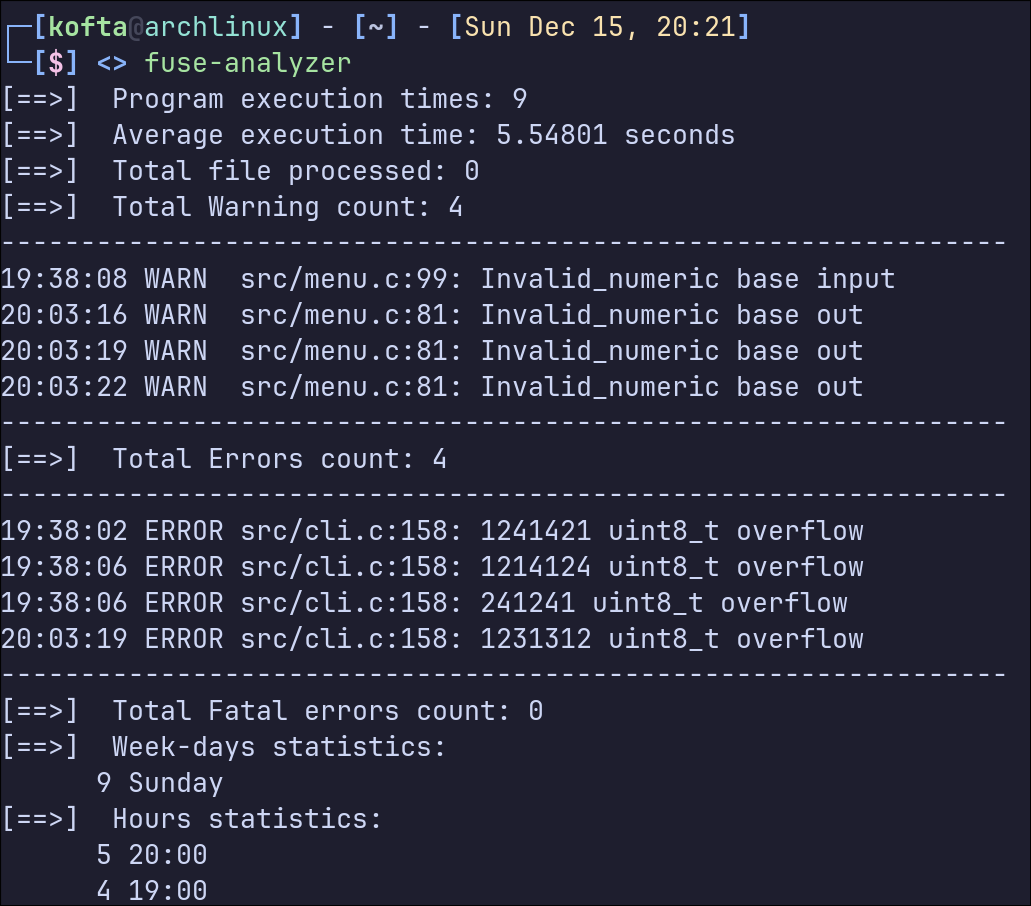
\includegraphics[width=0.75\textwidth]{assets/fuse-analyzer-default.png}
	\caption{Simple command, that analyze all \texttt{.log} files.}
\end{figure}

\newpage


\begin{figure}[h]
	\centering
	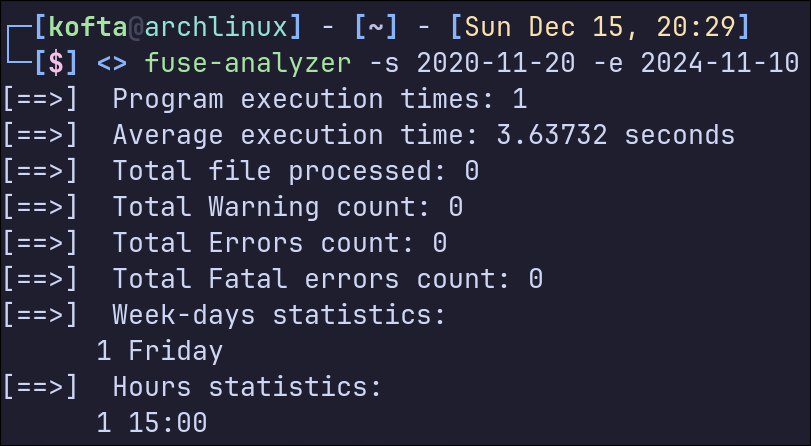
\includegraphics[width=0.75\textwidth]{assets/fuse-analyzer-data.png}
	\caption{Showing only data from 2020-11-20 up to 2024-11-10}
\end{figure}


\begin{figure}[h]
	\centering
	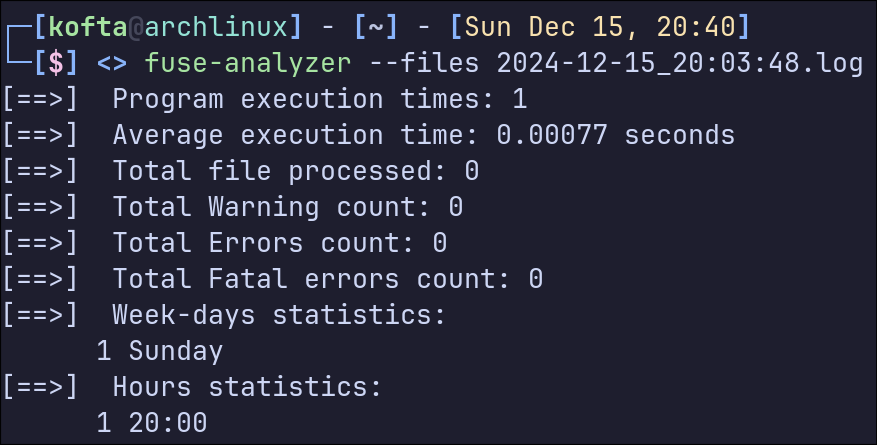
\includegraphics[width=0.75\textwidth]{assets/fuse-analyzer-files.png}
	\caption{Analyze only one file.}
\end{figure}

\section{Conclusion}
Fuse-analyzer provides a simple and convenient interface for viewing and analyzing log files generated during the interpreter's operations.




\vspace*{\fill}
\begin{center}Created in \raisebox{-0.5ex}{
\includegraphics[height=1em]{assets/linux.png}} \& \raisebox{-0.5ex}{
\includegraphics[height=1em]{assets/neovim.png}}
	with \raisebox{-0.5ex}{
\includegraphics[height=1em]{assets/love.png}}\end{center}

\end{document}
